\section{Auswertung}
\label{sec:Auswertung}
Die Graphen wurden sowohl mit Matplotlib \cite{matplotlib} als auch NumPy \cite{numpy} erstellt. Die
Fehlerrechnung wurde mithilfe von Uncertainties \cite{uncertainties} durchgeführt. Die Vermessung der Photographien wurde mit Gimp durchgeführt. Um die einzelnen Linien der Spektren besser zu erkennen wurden Kontrast, Helligkeit, Sättigung und Farbtiefe der Photographien für die Auswertung modifiziert.%cite gimp angeben



\subsection{Berechnung der theoretischen Landefaktoren für den normalen und anormalen Zeemanneffekt}
Zunächt werden die nach der Quantenmechanik theoretisch zu erwartenden Landefaktoren berechnet. Für die Aufspaltung der roten Linien des normalen Zeemanneffektes ist der Übergang zwischen $^1 D_2$ und $^1 P_1$ zu betrachten.
 Da der Spin Null ist, ergeben sich die drei in Abb. \ref{fig:normaleAufspaltung} dargestellten Fälle. Da nur eine longitudinale Betrachtung des Effektes erfolgt sind nur die beiden $\sigma$ Linien experimentell zu erkennen. Für diese liefert Formel \eqref{eq:LandeFaktor} in beiden Fällen $g_\text{j} = 1$.
Für die Aufspaltung der blauen Linien des anormalen Zeemanneffektes wird der Übergang zwischen $^3 P_1$ und $^3 S_1$ zu betrachtet. Bei diesem lassen sich über \eqref{eq:LandeFaktor} verschiedene Landefaktoren bestimmen. 
\begin{gather}
	0.5 (\pi)// 
	1.5 (\sigma)//
	2 (\sigma)
\end{gather}
Da die $\pi$ Linie nur einen geringen Landefaktor besitzt ist ein größeres Magnetfeld notwendig um die Aufspaltung sichtbar zu machen. Die beiden $\sigma$ Linie besitzen hingegen sehr ähnliche Landefaktoren, sodass experimentell eine gemeinsame Linie mit $g= 1.75$ zu erwarten ist.

\subsection{Kalibrierung des angelegten B-Feldes}

\begin{figure}
	\centering
	\includegraphics[width=\linewidth-70pt,height=\textheight-70pt,keepaspectratio]{build/Bfeldkali.pdf}
	\caption{Die Kalibrationskurve des B-Feldes in Abhängigkeit der Stromstärke.}
	\label{fig:BvonI}
\end{figure}

\begin{table}
	\centering
	\caption{Die genommenen Messwerte der B-Feldkalibrierung.}
	\input{build/tabIb1.tex}
	\input{build/tabIb2.tex}
	\label{tab:BvonI}
\end{table}

Zunächst wird die Stärke des B-Feld des Helmholtzspulenpaares, in dessen Zentrum sich die Cadmiumlampe befindet, in Abhängigkeit der angelegten Stromstärke vermessen. Es ergaben sich die Werte in Tabelle \ref{tab:BvonI}. Mithilfe einer lineare Ausgleichsrechnung der Form $a*x+b$ ergibt sich der Graph in Abb. \ref{fig:BvonI}. Für die beiden Konstanten $a$ und $b$ folgt: 
\begin{gather}
	a = \SI{0.0523(5)}{\tesla\per\ampere}%werte einfügen
	b = \SI{0.019(5)}{\tesla}
\end{gather}

\subsection{Vermessung des normalen Zeemanneffekts an der roten SIGMA Cadmiumlinie}

\begin{figure}
	\centering
	\includegraphics[width=\linewidth-70pt,height=\textheight-70pt,keepaspectratio]{content/Images/normalb0und1.jpg}
	\caption{Die Aufspaltung der Spektrallinien der roten $\sigma$ Cadmiumlinie.}
	\label{fig:normal}
\end{figure}

Nun wird der Landefaktor der roten $\sigma$ Cadmiumlinie bestimmt. Hierzu wurden die Photographien des Interferenzmusters mit und ohne B-Feld in Abb. \ref{fig:normal} aufgenommen. In diesem werden die Abstände zwischen den Ordnungen $\Delta s$und die Abstände der Aufspaltungen der einzelnen Ordnungen $\sigma s$ vermessen. Es ergeben sich die Abstände in den Tabellen \ref{tab:Deltas} und \ref{tab:sigmas}

Auf Basis von Formel \eqref{eq:} und Formel \eqref{} mit den Konstanten$\lambda = \SI{643.8}{\nano\meter}$ und $n = 1.4567$ ergeben sich die einzelnen $\Delta\lambda_\text{norm,\sigma}$ in Tabelle \ref{tab:deltsigmas}. Ein mittleres $\Delta\lambda$ wird über eine konstante Ausgleichsrechnung der Form $c$ zu $\SI{}{}$ bestimmt. Der Landefaktor berechnet mithilfe von Formel \eqref{} und bei einer angelegten Stromstärke von $\SI{9.5}{\ampere}$ %konstanten angeben
zu :::: . Zur Bestimmung des Magnetfeldes wurde die Kalibrierung verwendet, die Werte für $h$ und $c$ stammen aus \cite{scipy}% sind die konstanten auch von scipy?


\subsection{Vermessung des anormalen Zeemanneffekts an der blauen SIGMA Cadmiumlinie }

\begin{figure}
	\centering
	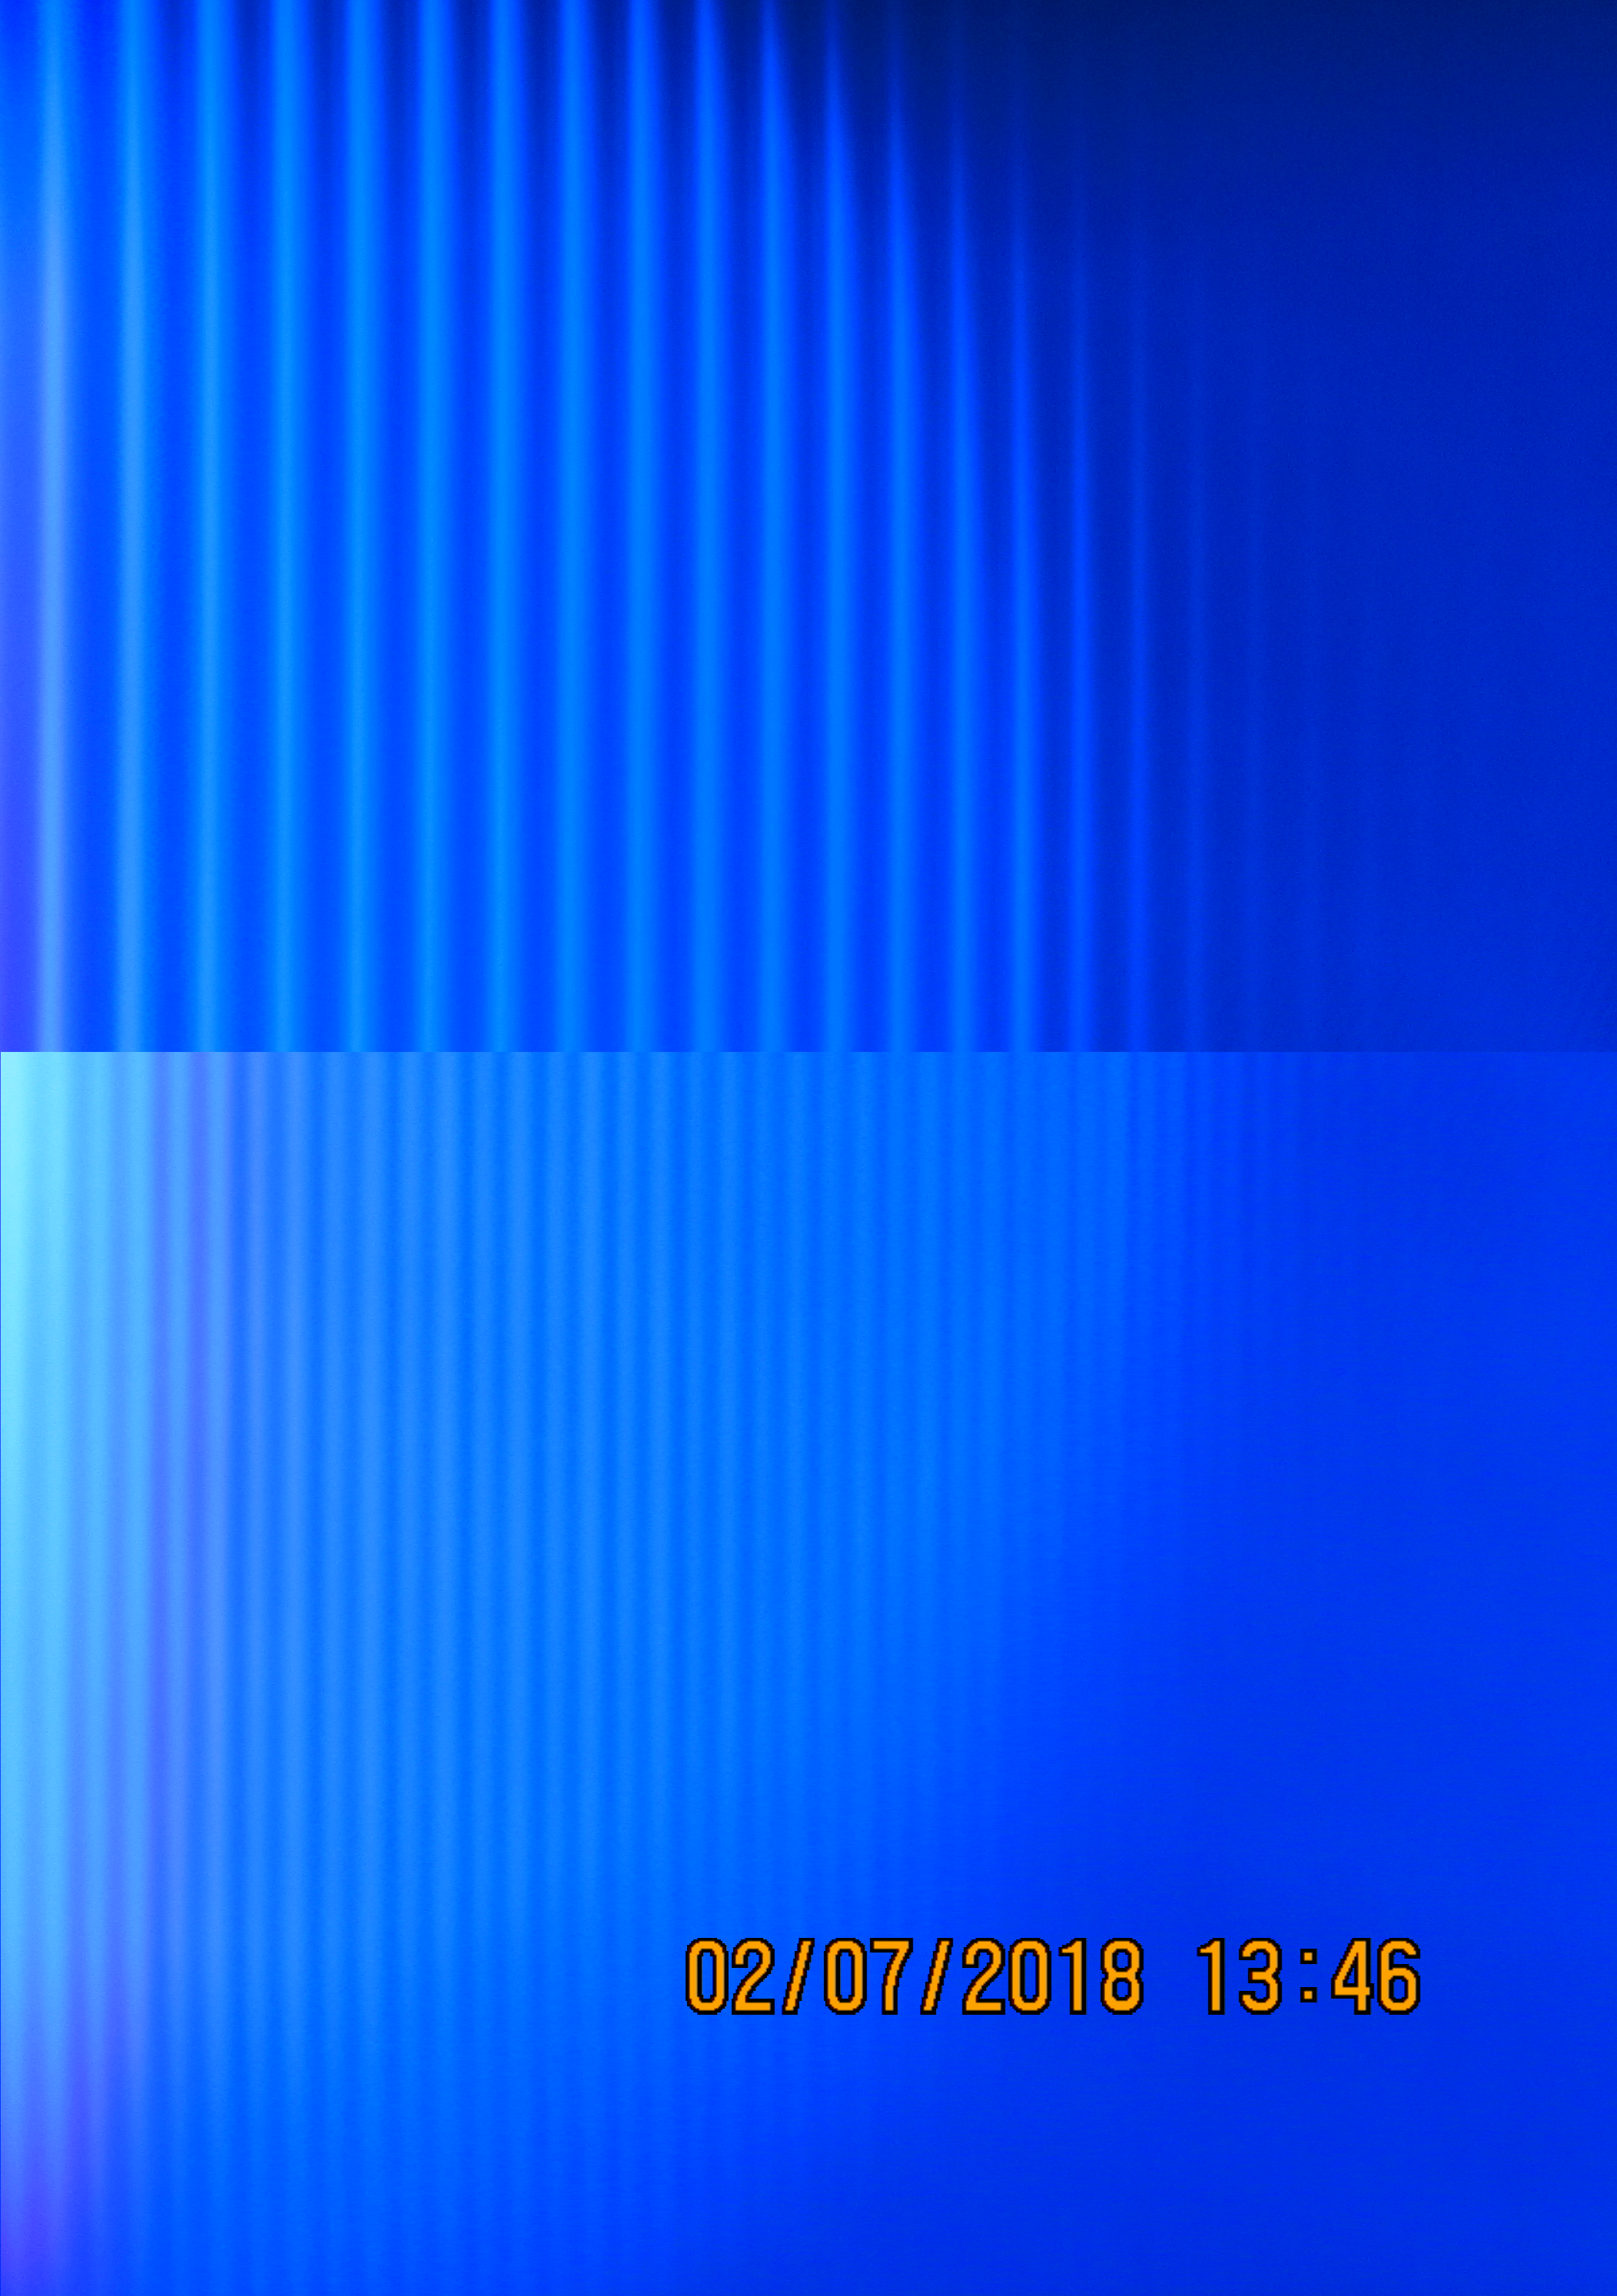
\includegraphics[width=\linewidth-70pt,height=\textheight-70pt,keepaspectratio]{content/Images/annormalsigmab0und1.png}
	\caption{Die Aufspaltung der Spektrallinien der blauen $\sigma$ Cadmiumlinie.}
	\label{fig:anormal1}
\end{figure}


Der bereits für den normalen Zeemanneffekt beschriebene Vorgang wird nun für die blaue $\sigma$ Cadmiumlinie wiederholt. Aus der Photographie \ref{fig:} konnten die Abstände in den Tabellen \ref{tab:Deltas} und \ref{tab:sigmas} bestimmt werden. Zur Bestimmung von $\Delta\lambda_\text{anorm,\sigma}$ werden diesmal die Konstanten $\SI{480}{\nano\meter}$ und $n = 1.4635$ verwendet. Es ergeben sich die Werte in Tabelle \ref{tab:deltsigmas}. Das mittleres $\Delta\lambda_\text{anorm,\sigma}$ wird zu $\SI{}{}$ bestimmt. Der Landefaktor berechnet sich bei einer angelegten Stromstärke von $\SI{5.9}{\ampere}$ %konstanten angeben
zu :::: .



\subsection{Vermessung des anormalen Zeemanneffekts an der blauen PI Cadmiumlinie}

Das Verfahren wird ein letztes Mal für die blaue $\pi$ Cadmiumlinie angewendet. Aus der Photographie \ref{fig:} konnten die Abstände in den Tabellen \ref{tab:Deltas} und \ref{tab:sigmas} bestimmt werden.  Daraus folgen die $\Delta\lambda_\text{anorm,\pi}$ in Tabelle \ref{tab:deltsigmas}. Die Konstanten bleiben diesselben wie bei den anormalen $\sigma$ Linien. Der Landefaktor berechnet sich bei einer angelegten Stromstärke von $\SI{16.25}{\ampere}$ %konstanten angeben
zu :::: .

\begin{figure}
	\centering
	\includegraphics[width=\linewidth-70pt,height=\textheight-70pt,keepaspectratio]{content/Images/pianormalB0und1.jpg}
	\caption{Die Aufspaltung der Spektrallinien der blauen $\pi$ Cadmiumlinie.}
	\label{fig:anormal2}
\end{figure}


\subsection{Tabellen}

\begin{table}
	\centering
	\caption{Die gemessenen Abstände zwischen den unterschiedlichen Ordnungen aus den Photographien ohne angelegtes B-Feld..}
	\input{build/tabdelta.tex}
	\label{tab:Deltas}
\end{table}

\begin{table}
	\centering
	\caption{Die gemessenen Abstände der Aufspaltungen aus den Photographien mit angelegtem B-Feld.}
	\input{build/tabsigma.tex}
	\label{tab:sigmas}
\end{table}

\begin{table}
	\centering
	\caption{Die bestimmten $\Delta\lambda$ der verschiedenen Aufnahmen.}
	\input{build/deltalambda.tex}
	\label{tab:deltsigmas}
\end{table}